\begin{figure}
  \centering
  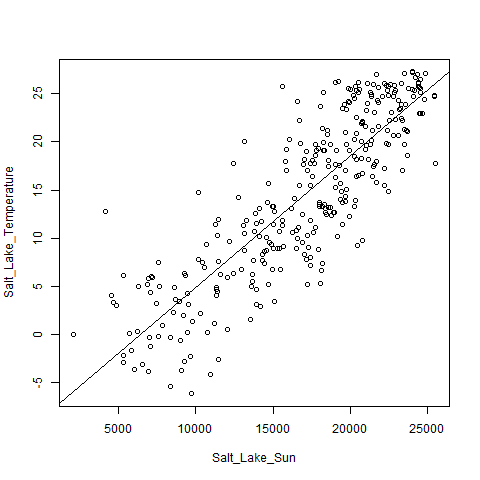
\includegraphics[width=7cm]{../data/img/Temp_vs_sun.PNG}
  \caption{Salt Lake City Temperature versus Sun}
  \label{fig:temp_vs_sun}
\end{figure}

\begin{figure}
  \centering
  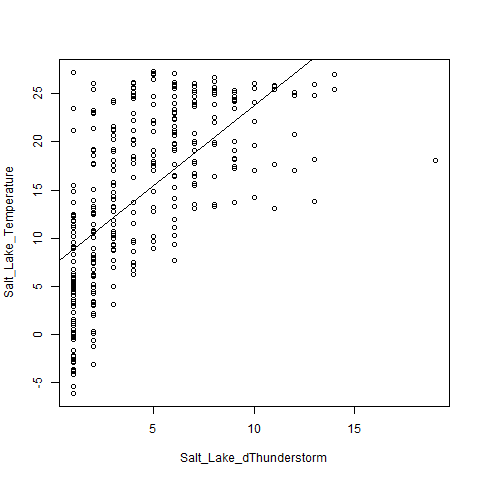
\includegraphics[width=7cm]{../data/img/Temp_vs_dThunderstorm.PNG}
  \caption{Salt Lake City Temperature versus Days of Thunderstorms}
  \label{fig:temp_vs_dthunderstorms}
\end{figure}

\begin{figure}
  \centering
  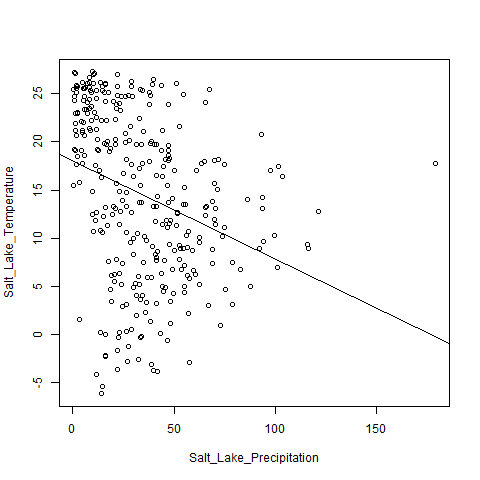
\includegraphics[width=7cm]{../data/img/Temp_vs_Precipitation.PNG}
  \caption{Salt Lake City Temperature versus Precipation}
  \label{fig:temp_vs_precipation}
\end{figure}

\begin{figure}
  \centering
  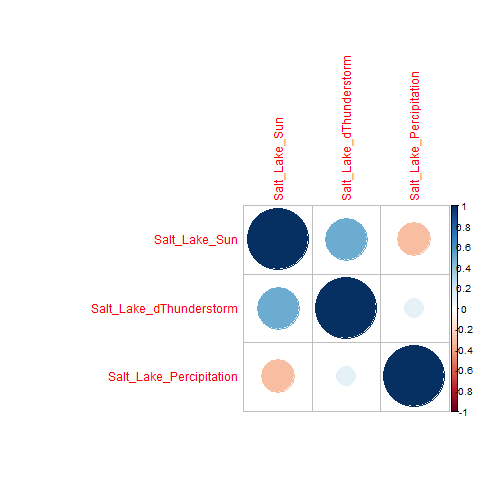
\includegraphics[width=7cm]{../data/img/correlation_plot.PNG}
  \caption{Correlation plot of chosen dependent variables}
  \label{fig:correlation_plot}
\end{figure}

\begin{table}[ht]
 \begin{centering}
 \begin{tabular}{|c|c c c c c|} 
 \hline
 $$ & & & & Days of & \\ [0.5ex] 
 & Temperature & Intercept & Minutes of Sun & Thunderstorms & Precipitation \\
 \hline\hline
 $P_{Shapiro}$ & $2.662\times 10^{-8}$ & -- & $6.845\times 10^{-9}$ & $9.438\times 10^{-15}$ & $2.817\times 10^{-12}$ \\ 
 \hline
 $\beta$ & -- & -5.261 & $1.041\times 10^{-3}$ & 0.8471 & $-4.800\times 10^{-2}$ \\ 
 \hline
 $P(>|t|)$ & -- & $2.30\times 10^{-8}$ & $< 2.00\times 10^{-16}$ & $< 2.00\times 10^{-16}$ & $< 2.91\times 10^{-7}$ \\ 
 \hline
 \end{tabular}
 \caption{Multilinear Regression for Predicting Temperature (Adjusted $R^{2} = 0.7969$, $n = 321$)}
 \label{tab:lin_regression}
 \end{centering}
\end{table}

\begin{table}[ht]
 \begin{centering}
 \begin{tabular}{|c|c c c|} 
 \hline
  \# Variables & Minutes of Sun & Days of Thunderstorms & Precipitation \\
 \hline
 1 & * & & \\
  \hline
 2 & * & * & \\ 
  \hline
 3 & * & * & *\\ 
 \hline
 \end{tabular}
 \caption{Optimal Subset selection for Multilinear Regression}
 \label{tab:optimal_selection}
 \end{centering}
\end{table}